\documentclass[a4paper]{article}
\usepackage[a4paper, total={6in, 15in}]{geometry}
\usepackage{siunitx}
\usepackage{physics}
\usepackage{amsmath}
\usepackage{amssymb}
\usepackage{listings}
\usepackage{color}
\usepackage{hyperref}
\usepackage{titling}
\usepackage{epsfig}
\usepackage{ison2022}
\graphicspath{{report/}} 
\definecolor{pythonred}{rgb}{0.6,0,0} % for strings
\definecolor{pythongreen}{rgb}{0.25,0.5,0.35} % comments
\definecolor{pythonpurple}{rgb}{0.5,0,0.35} % keywords
\definecolor{pythondocblue}{rgb}{0.25,0.35,0.75} % pythondoc
\lstset{language=Python, basicstyle=\ttfamily,
keywordstyle=\color{pythonpurple}\bfseries, stringstyle=\color{pythonred},
commentstyle=\color{pythongreen},
morecomment=[s][\color{pythondocblue}]{/**}{*/}, tabsize=4, showspaces=false,
basicstyle=\fontsize{9}{9}\selectfont\ttfamily, showstringspaces=false}


\title{Vela Partners: Twins Project}
\name{Ian Cheung, Keble College}
\setlength{\parindent}{0pt}
\setcounter{tocdepth}{2}

\begin{document}
\maketitle
\tableofcontents
\section{Abstract}
We use 
\section{Introduction}
When there is a window of opportunity, smart entrepreneurs all around the world
seek the same opportunities. For that reason, there is almost never only one
company tackling a problem. In this project, our goal is to build a model to
find similar companies when a company is given as an input.
\subsection{Data}
The dataset contains 655,000 companies and contains the description of the
what the companies do, along with a category label. There are around 55,000
unique categories, and a median of 10 companies per category.
\subsection{Aims and approach}

\begin{figure}[!h]
    \centerline{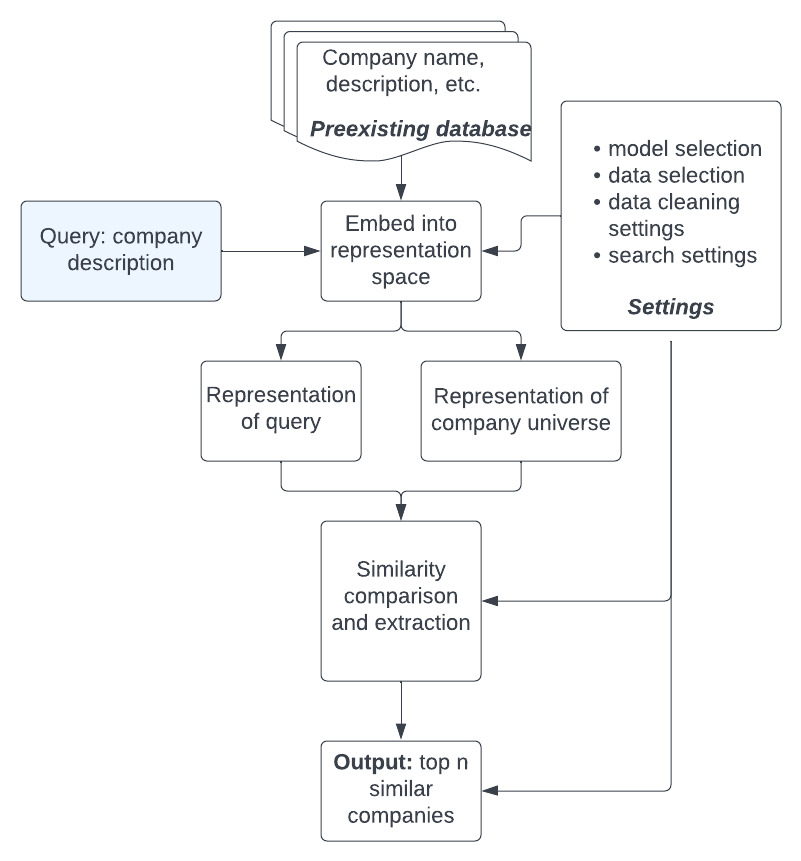
\includegraphics[width=95mm]{uml.jpeg}} \caption{{\it UML diagram}[\ref{uml}]}
    \label{setup}
\end{figure}

\clearpage
\begin{thebibliography}{9}
\bibitem{cmanual}Perez-Callejo et al., \emph{X-ray Spectroscopic Studies of a Solid-Density
Germanium Plasma Created by a Free Electron Laser}, Applied Sciences,
2020\label{sampaper} 
\end{thebibliography}


\appendix
\renewcommand\thesection{Appendix \Alph{section}}
\end{document}